\section{Strukturiert}
Im Folgenden wird beschrieben, wie das strukturierte Netz der Aachen-Turbine erstellt wurde. Da das Netz Einfluss auf die numerische Konvergenz der Lösungsverfahren, auf die Qualität der Lösung, auf die Auflösung und damit auch auf den Diskretisierungsfehler hat, ist ein gutes Netz von großer Bedeutung. Deshalb wurde eine Netzstudie - basierend auf einem Referenzgitter – durchgeführt und anschließend das bestmögliche Netz in Bezug auf Qualität vs. geringe Anzahl an Gitterzellen ausgewählt. 

\subsection{Erstellung des Gitters}

Zunächst wurde das Referenzgitter erstellt. Dazu wurde die Geometrie der Aachen-Turbine mittels des strukturierten Multi-Block Netzgenerators AutoGrid5 vernetzt. Dieser ist speziell für die Vernetzung von Turbomaschinen ausgelegt. 
Da die uns zur Verfügung stehende Vorlage der Aachen-Turbine die 1,5 Stufen zusammenhängend beinhaltete, erzeugten wir zu Beginn jeweils einzelne Gitter für Stator1, Rotor und Stator2 um diese später in CFX verwenden zu können. Hierbei wurde jeweils erst ein Vernetzungsdurchlauf basierend auf den voreingestellten Standartwerten durchgeführt und anschließend manuell optimiert. Für eine ausreichend gute Netzqualität dürfen bestimmte Netzkriterien nicht verletzt werden. Andernfalls kann es sein, dass die Lösung nicht, oder nur schlecht konvergiert. In unserem Fall haben wir darauf geachtet, dass wir keine negativen Kontrollvolumina haben, dass die kleinsten Winkel in einer Zelle größer 20° sind, dass das Expansionratio - welches das Volumenverhältnis zweier Zellen beschreibt – kleiner als 2.3 ist und dass das Aspectratio – welches das Verhältnis von längster zu kürzester Seite einer Zelle angibt – unter 1500 ist. Variiert wurden hauptsächlich die Anzahl und die Verteilung der Zellen in der B2B Ansicht. Diese stellt einen Querschnitt durch die Schaufel dar. In radialer Richtung wurde die Zellenverteilung im „flowpath“ angepasst. 

\subsection{Spaltverfeinerung}

Zur Bestimmung der Gitterauflösung im Spalt des Rotors wurde zudem die Anzahl der Zellen im Spalt variiert. Es stellte sich heraus, dass im Vergleich zum ursprünglichen Gitter mehr Zellen hinzugefügt werden mussten, da die Auflösung nicht fein genug war und man Änderungen im Vergleich zur gröberen Auflösung sah.  In den Abbildungen \ref{effSpalt1} und \ref{effSpalt15} ist die Gitterstudie für den Spalt mit 1 und 1,5 Stufen dargestellt. \todo welches Gitter ausgewählt, 3.?


%\begin{figure}[htbp]
%	\centering
%	\label{effSpalt1}
%	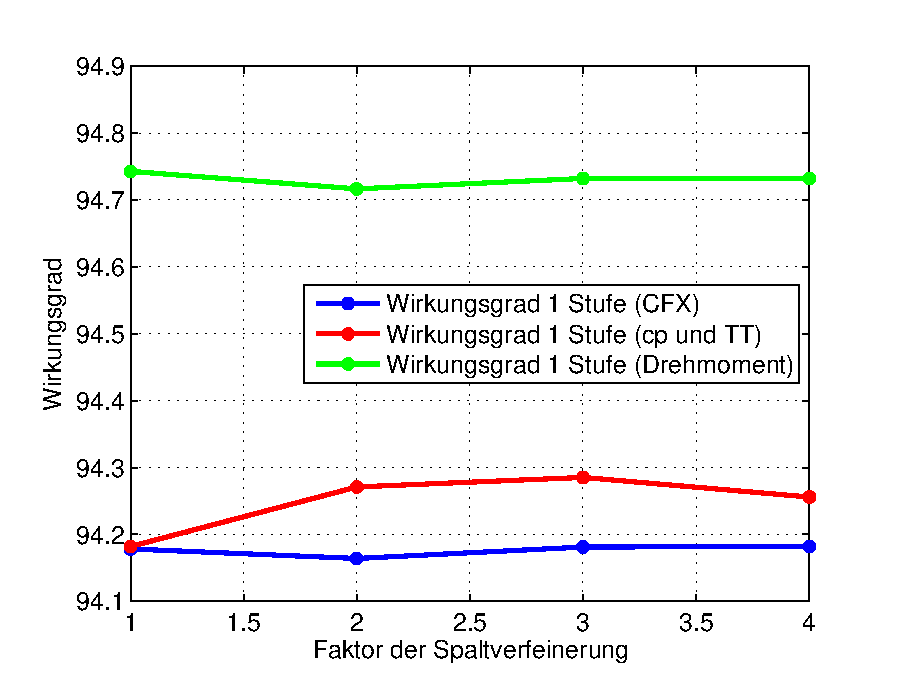
\includegraphics[width=0.7\textwidth]{efficiencySpalt1Stufe.eps}
%	\caption{Gitterstudie des Spalts für eine Stufe}
%\end{figure}
%
%\begin{figure}[htbp]
%	\centering
%	\label{effSpalt15}
%	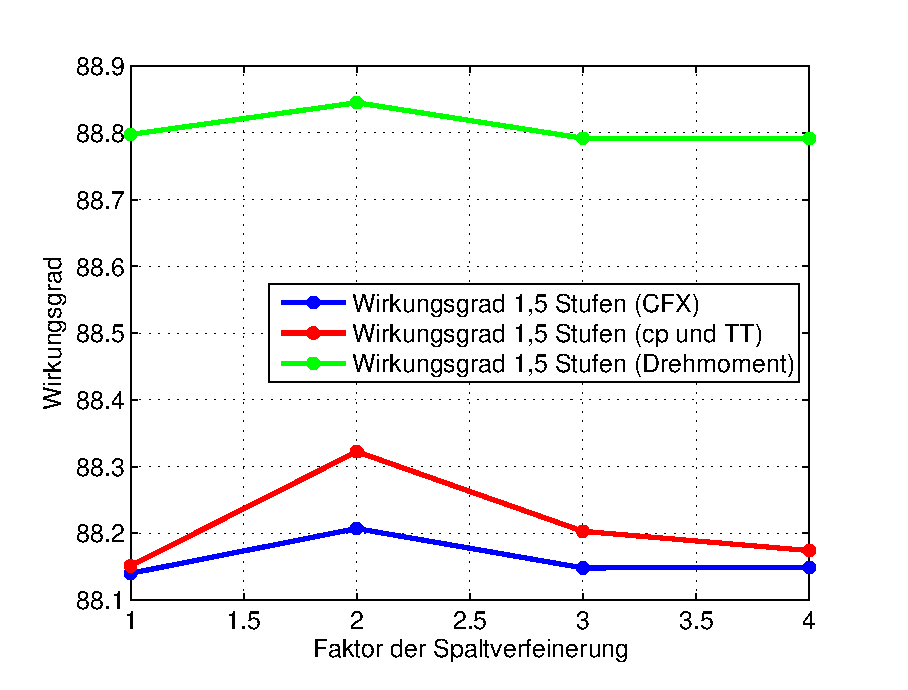
\includegraphics[width=0.7\textwidth]{efficiencySpalt15Stufen.eps}
%	\caption{Gitterstudie des Spalts für 1,5 Stufen}
%\end{figure}

\subsection{Einstellen der Grenzschichtdicke}
Außerdem musste noch die Grenzschichtdicke, bzw. das y-plus eingestellt werden. Die Strömung wurde bis in die viskose Unterschicht aufgelöst, sodass die Auflösung in Wandnähe im Bereich der kleinsten Wirbel liegt. Das Verhältnis der Grenzschichtdicke zu den kleinsten Wirbeln sollte kleiner als 1 sein. \todo Formel einfügen. Um das korrekte y-plus zu bestimmen, haben wir die Werte in AutoGrid für den Wandabstand sowohl auf dem Schaufelrand im B2B-Layer, als auch an Hub und Shroud variiert.  Anschließend haben wir eine Simulation in CFX durchgeführt und dann die Verteilung des y-plus-Wertes über die Schaufel hinweg visualisiert und ausgewertet. Schließlich kamen wir zu dem Ergebnis, dass die optimale Grenzschichtdicke für den Rotor bei $2e-6$ im Flowpath an Hub und Shroud und bei $1.5e-6$ am Blade liegt. Die kompletten Werte sind in Tabelle \ref{cellWidths} zu sehen. Über die komplette Schaufel betrachtet liegen die y-plus-Werte in einem Bereich von $0.3 \leq y^+ \leq 3$ nahezu überall. Da man nur wenige Stellschrauben zur Beeinflussung dieses Wertes in AutoGrid hat, ist dieser Wertebereich zufriedenstellend, zumal die Mehrheit der Werte im Bereich von $0.7 \leq y^+ \leq 1.2$  liegt, wie in Abb. \ref{imgYplusWerte} zu sehen ist. 

\begin{table}[t]
\centering
\begin{tabular}[t]{cccc}
\toprule
 Cell width  & Stator1 & Rotor & Stator2  \\
\midrule
Cell width at Hub & 2.7e-6 & 2e-6 & 1.4e-6\\
Cell width at Shroud & 2.7e-6 & 2e-6 & 1.4e-6 \\
Cell width at Wall (Blade) & 1.56e-6 & 1.5e-6 & 1.7e-6 \\
\bottomrule
\end{tabular}
\caption{Zellgrößen an der Wand für Rotor und die Statoren}
\label{cellWidths}
\end{table}

\begin{figure}[htbp]
	\centering
	\label{imgYplusWerte}
	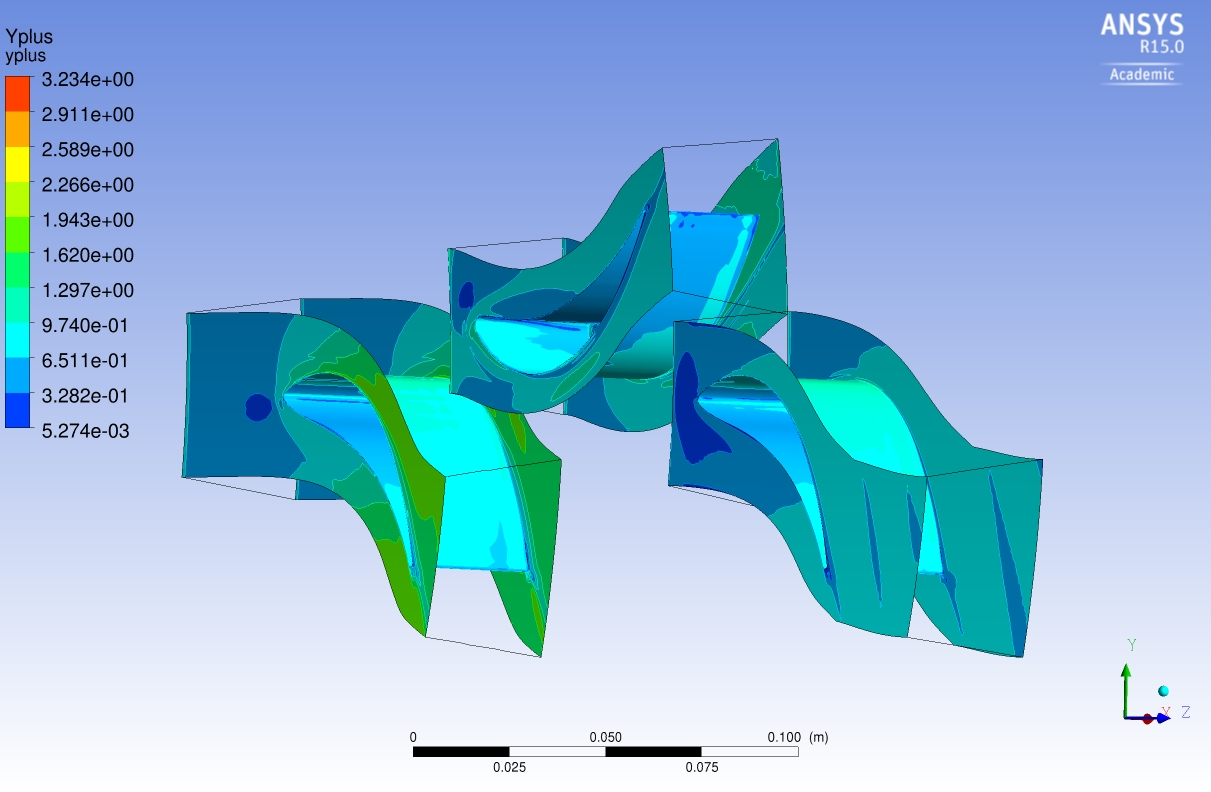
\includegraphics[width=0.7\textwidth]{yPlus.jpg}
	\caption{$y^+$-Verteilung über die komplette Stufe}
\end{figure}

\subsection{Durchführung der Netzstudie}

Nachdem nun ein Referenzgitter mit guter Gitterqualität und korrekter Grenzschichtdicke vorhanden war, konnte die eigentliche Netzstudie durchgeführt werden um die minimale Auflösung zu bestimmen, die das Netz haben muss, damit die Lösung netzunabhängig ist. Hierzu wurde das Referenzgitter sowohl gröber aufgelöst, als auch verfeinert und dann der Einfluss auf verschiedene Größen, die z.B. die Wirkungsgrade verglichen. Sobald sich dieser im Vergleich zum nächst feineren, bzw. nächst gröberen Gitter kaum noch ändert, ist die Lösung von der Gitterdiskretisierung unabhängig. 
Insgesamt wurden 7 verschiedene Verfeinerungsstufen erstellt und simuliert. Das Referenzgitter hat jeweils knapp 1 Million Zellen für Rotor und die Statoren. Zunächst wurde versucht, die Zellenanzahl zu verdoppeln. Dazu wurde die Auflösung in allen drei Raumrichtungen mit $\sqrt[3]{2}$ multipliziert um insgesamt einen Faktor von 2 zu erlagen. Dies wurde dann nochmal wiederholt, um einen Faktor 4 gegenüber dem Referenznetz zu erreichen. Außerdem wurde das Referenznetz auf die halbe Zellenanzahl halbiert. Mit den Ergebnissen, dieser 4 Simulationen wurde bereits versucht, eine Aussage über die Netzunabhängigkeit zu treffen. Allerdings war hier noch nicht ganz ersichtlich, welches Netz hier genommen werden konnte, da die Unterschiede noch zu groß waren. Allerdings sah das 2x Gitter schon sehr gut aus. Daraufhin führten wir noch drei weitere Simulationen durch, jeweils mit den Auflösungen 1.3x, 1.5x und 3x in Bezug zum Referenzgitter. Nun war zu erkennen, dass das Netz mit der doppelten Auflösung praktisch unabhängig war, sodass wir dieses als unser Gitter für die nachfolgenden Rechnungen definieren konnten. 
\todo Kenngrößen des Gitters hinschreiben + Plots einfügen


\subsection{Fillets}

In realen Turbinen befinden sich an der Schaufel am Übergang zum Randbereich sogenannte Fillets, also Verrundungen, um bessere Strömungseigenschaften zu erhalten, Ablöseblasen zu vermeiden und bessere Festigkeitseigenschaften zu erhalten. Daher wurde auch eine Simulation der Aachen-Turbine mit Fillets durchgeführt, das Netz ist in Abb. \ref{imgFillet1} zu sehen. Jedoch ergab sich das Problem, dass nur sehr kleine Fillets erstellt werden konnten, da die Statoren eine „Delle“ an der Vorderkante aufweisen, wie in Abb. \ref{imgFilletDelle} zu sehen ist und daher ab einem bestimmten Radius negative Kontrollvolumen durch die Fillets entstehen. Jedoch wurde eine Simulation mit einem Fillet des Radius 0.00055 durchgeführt. Es hat sich herausgestellt, dass die Gitterqualität wesentlich schlechter wurde, da mehr schrägwinklige Zellen im Filletbereich notwendig wurden. Allerdings wurde auch der y-plus-Wertebereich etwas besser, da sehr kleine und sehr große Werte verschwanden.     

  \begin{figure}[htbp]
	\centering
	\label{imgFillet1}
	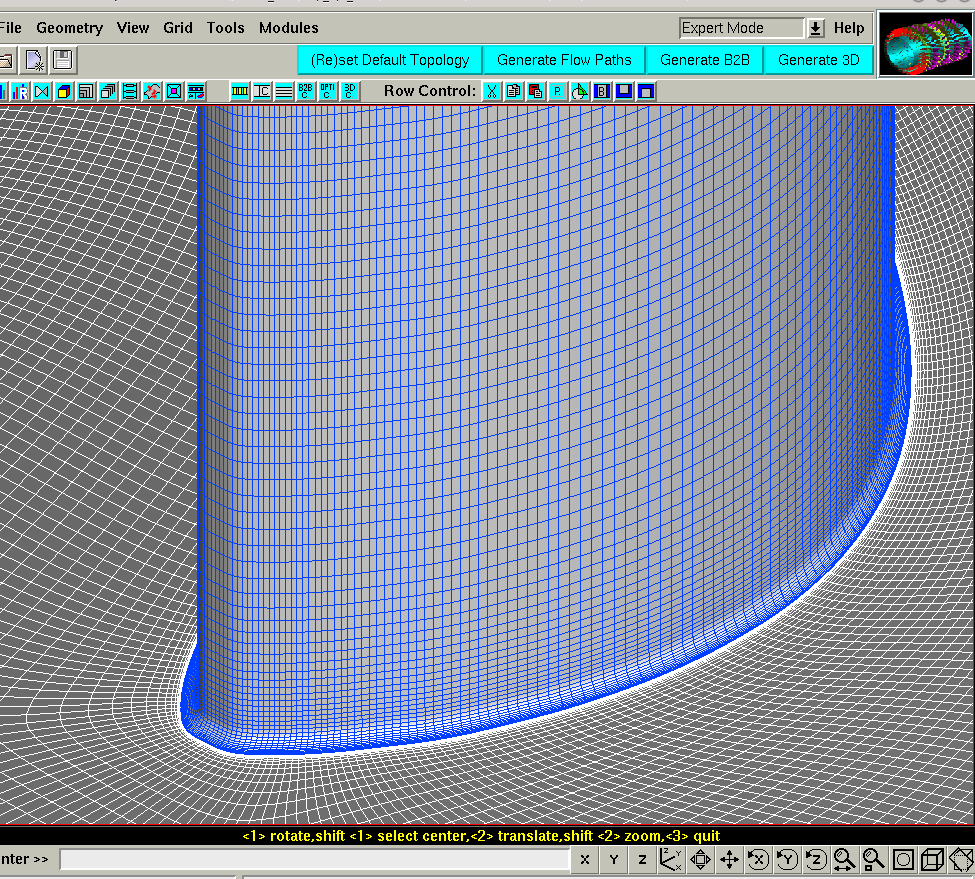
\includegraphics[width=0.7\textwidth]{fillet0_00055.png}
	\caption{Netz mit Fillet der Größe 0.00055}
\end{figure} 

  \begin{figure}[htbp]
	\centering
	\label{imgFilletDelle}
	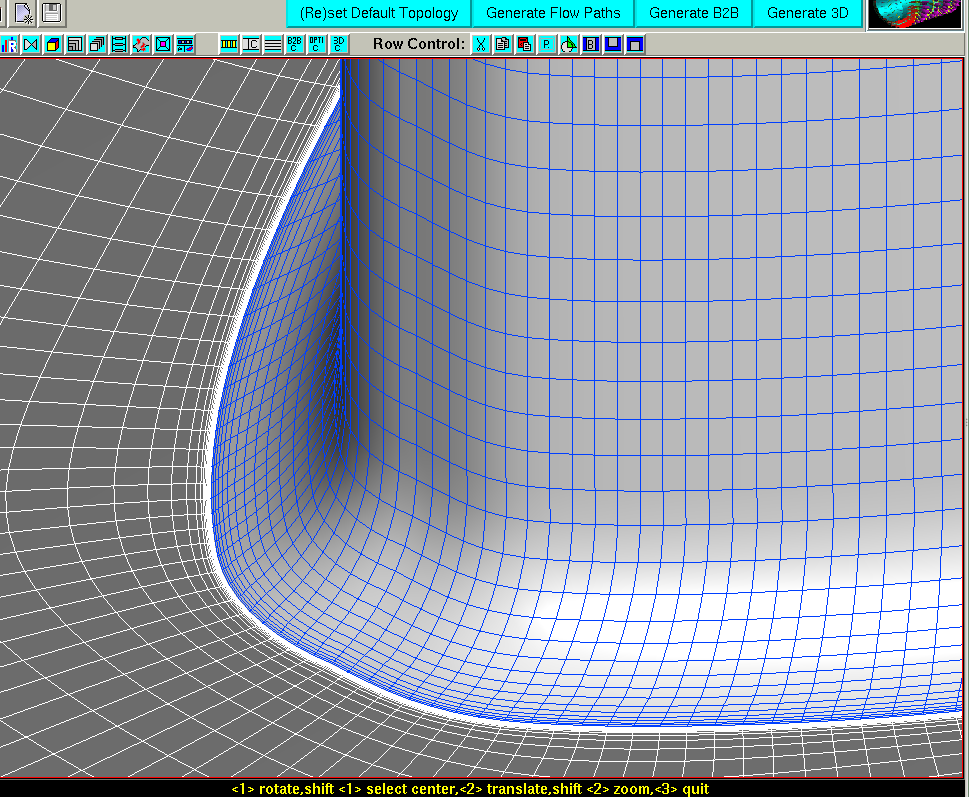
\includegraphics[width=0.7\textwidth]{filletDelle.png}
	\caption{Delle in der Statorgeometrie}
\end{figure} 